\documentclass[14pt]{article}
\title{Lab1 Report}
\author{Zepeng Chen}
\date{\today}
\usepackage{listings}
\usepackage{color}
\usepackage{graphicx}
\usepackage{subcaption}
\usepackage{gensymb}
\usepackage{geometry}
\geometry{a4paper,left=2cm,right=2cm,top=1cm,bottom=1cm}

\definecolor{dkgreen}{rgb}{0,0.6,0}
\definecolor{gray}{rgb}{0.5,0.5,0.5}
\definecolor{mauve}{rgb}{0.58,0,0.82}

\lstset{frame=tb,
	language=Matlab,
	aboveskip=3mm,
	belowskip=3mm,
	showstringspaces=false,
	columns=flexible,
	basicstyle={\small\ttfamily},
	numbers=none,
	numberstyle=\tiny\color{gray},
	keywordstyle=\color{blue},
	commentstyle=\color{dkgreen},
	stringstyle=\color{mauve},
	breaklines=true,
	breakatwhitespace=true,
	tabsize=3
}

\begin{document}
	\maketitle
	\tableofcontents
	\section{Basic Transformation}
	\subsection{Code Except Translation}
	\lstinputlisting[breaklines]{showFig.m}
	\subsection{Code For Translation}
	\lstinputlisting[breaklines]{translation.m}
	\subsection{Code For Rotation Followed by Translation}
	\lstinputlisting{rotAndtrans.m}
	\subsection{Code For Comparison between Built-in and Self-defined Rotation}
	\lstinputlisting{maketform.m}
	\newcommand{\RNum}[1]{\uppercase\expandafter{\romannumeral #1\relax}}
	\subsection{Outcome Set \RNum{1}}
	\newpage
	\begin{figure}[hbt!]
		\centering
		\begin{subfigure}[b]{0.23\linewidth}
			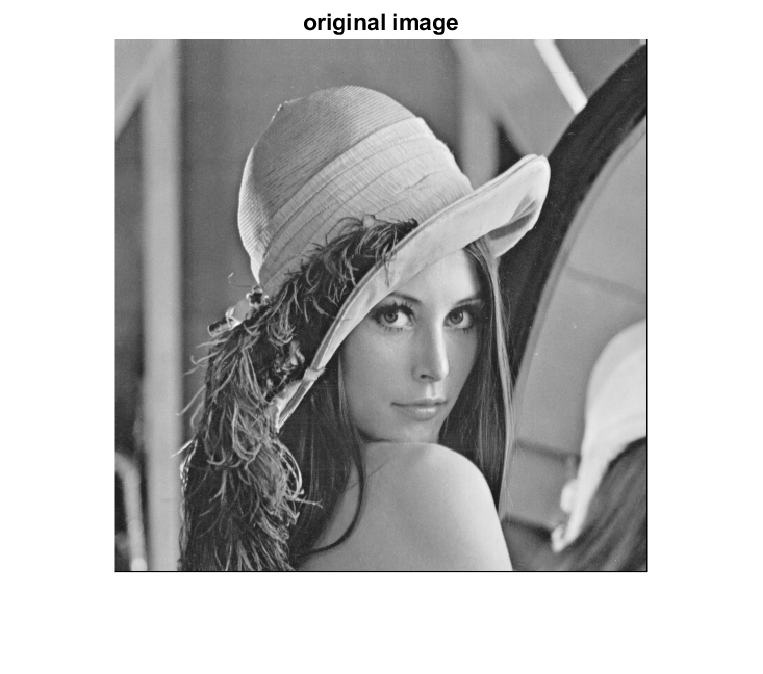
\includegraphics[width=\linewidth]{origin.png}
			\caption{Original Image.}
		\end{subfigure}
		\begin{subfigure}[b]{0.23\linewidth}
			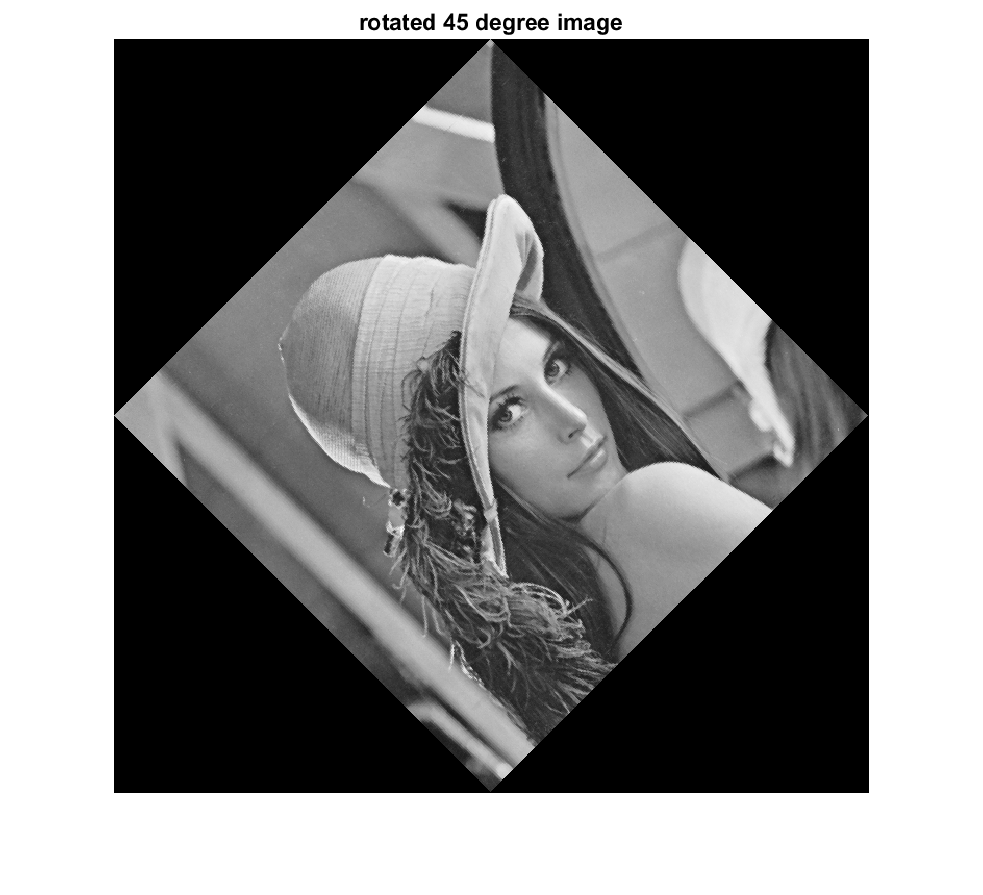
\includegraphics[width=\linewidth]{rot45.png}
			\caption{Rotate 45 \degree.}
		\end{subfigure}
		\begin{subfigure}[b]{0.23\linewidth}
			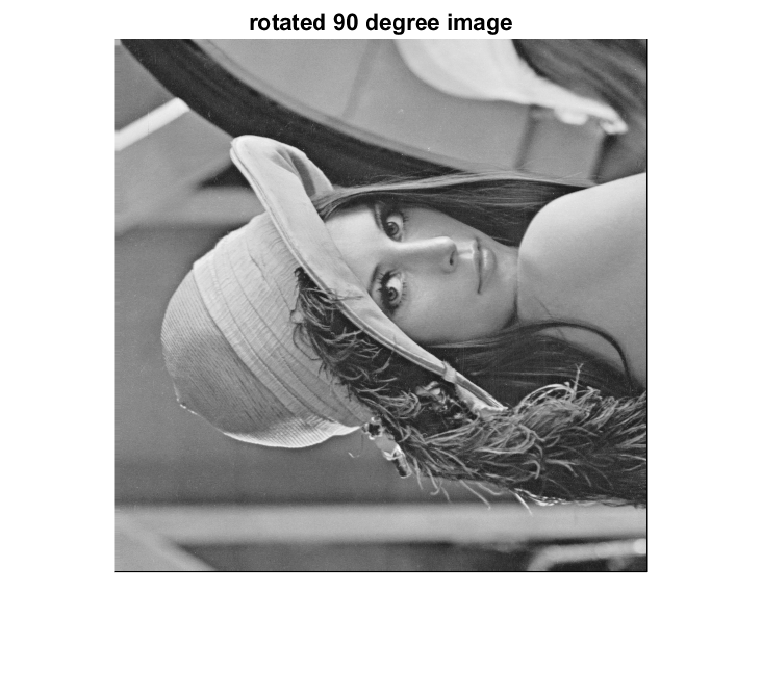
\includegraphics[width=\linewidth]{rot90.png}
			\caption{Rotate 90 \degree.}
		\end{subfigure}
		\begin{subfigure}[b]{0.23\linewidth}
			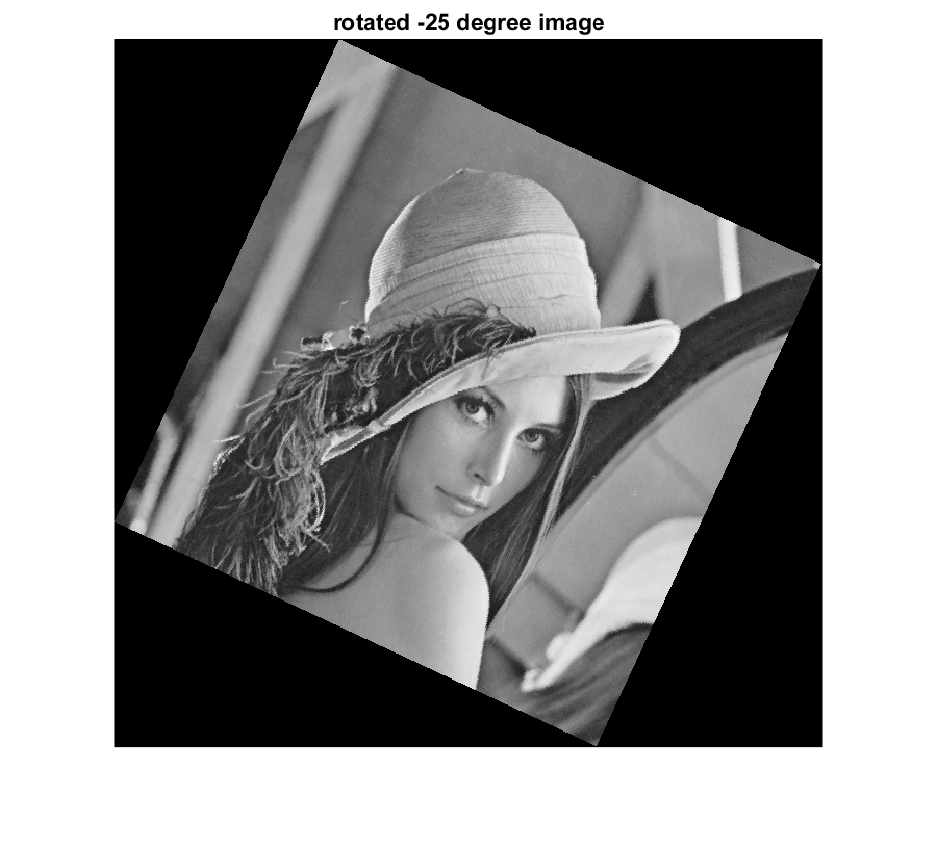
\includegraphics[width=\linewidth]{rot-25.png}
			\caption{Rotate -25 \degree.}
		\end{subfigure}
		\begin{subfigure}[b]{0.23\linewidth}
			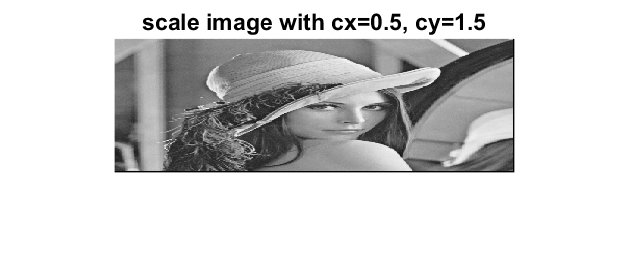
\includegraphics[width=\linewidth]{scale.png}
			\caption{Scale with cx=0.5, cy=1.5.}
		\end{subfigure}
		\begin{subfigure}[b]{0.23\linewidth}
			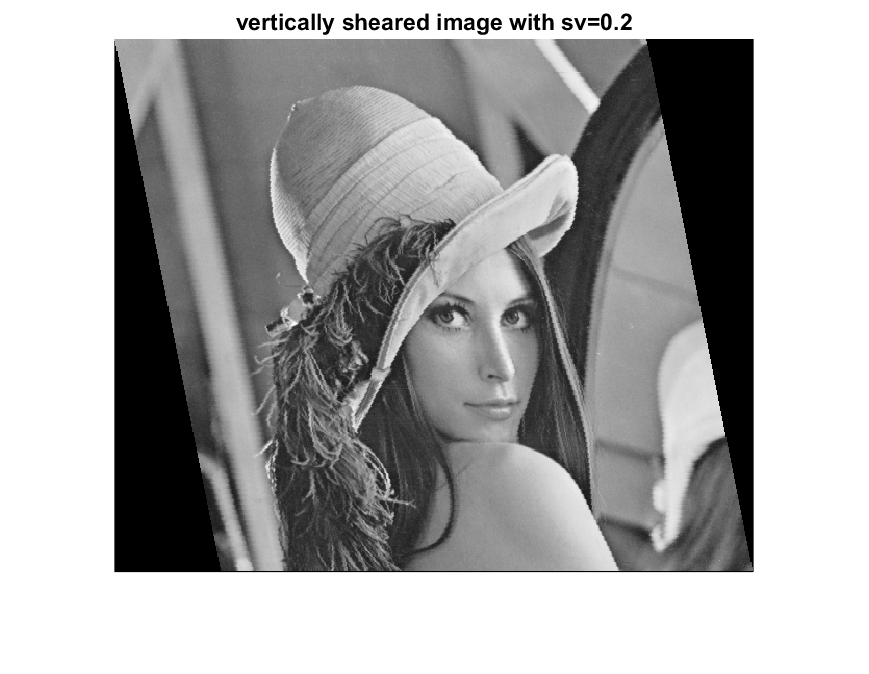
\includegraphics[width=\linewidth]{Vshear.png}
			\caption{Vertical shear with sv=0.2.}
		\end{subfigure}
		\begin{subfigure}[b]{0.23\linewidth}
			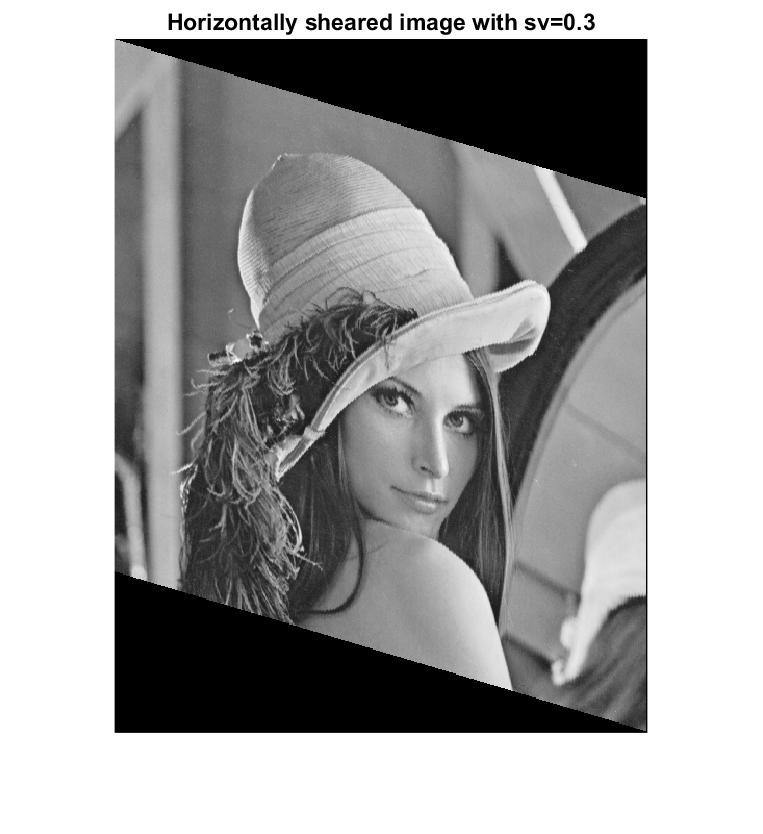
\includegraphics[width=\linewidth]{Hshear.png}
			\caption{Horizontal shear with sv=0.3.}
		\end{subfigure}
		\begin{subfigure}[b]{0.23\linewidth}
			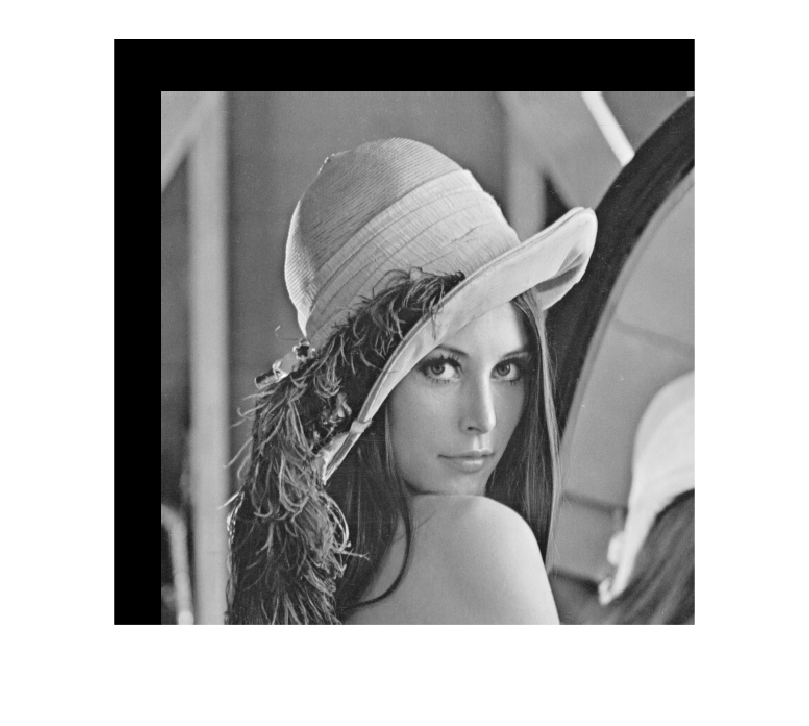
\includegraphics[width=\linewidth]{trans50-45.png}
			\caption{Translate with tx=50,ty=45.}
		\end{subfigure}
		\begin{subfigure}[b]{0.23\linewidth}
			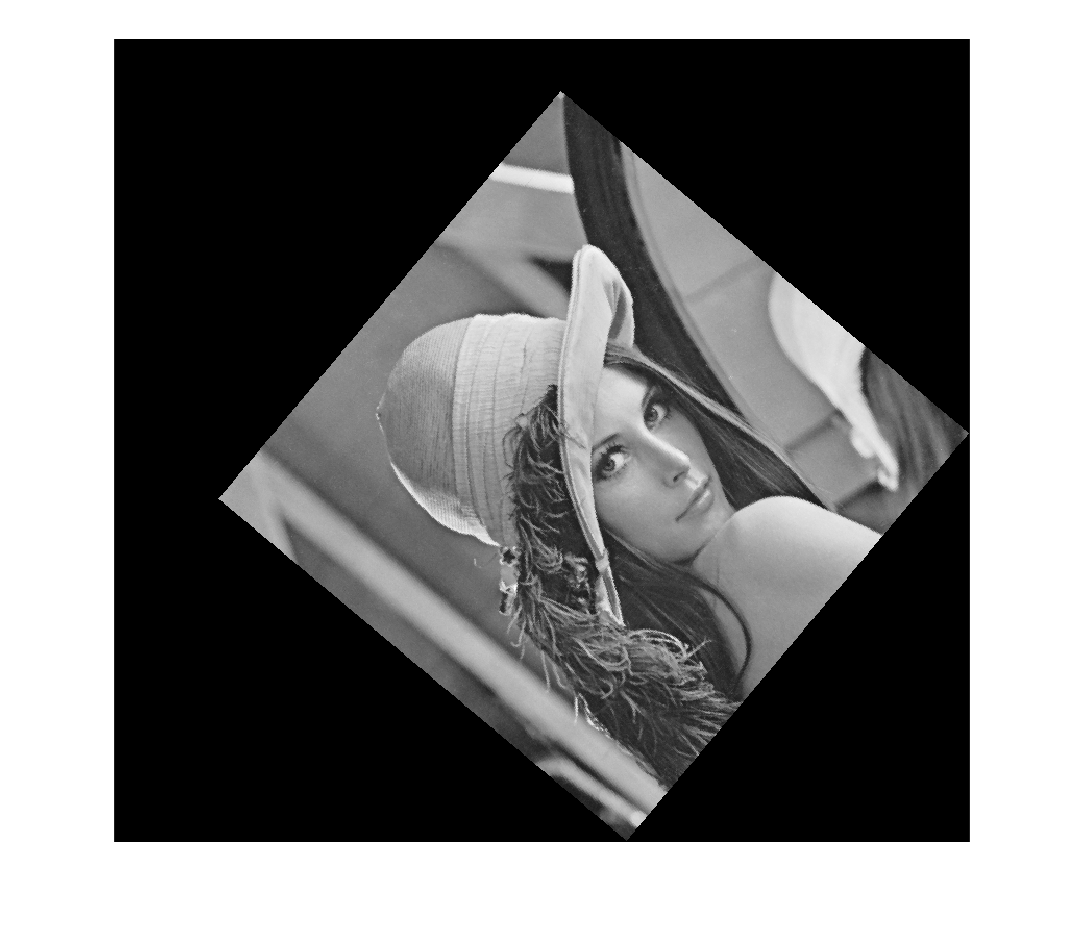
\includegraphics[width=\linewidth]{rotAndtrans.png}
			\caption{Rotation followed by translation.}
		\end{subfigure}
		\begin{subfigure}[b]{0.92\linewidth}
			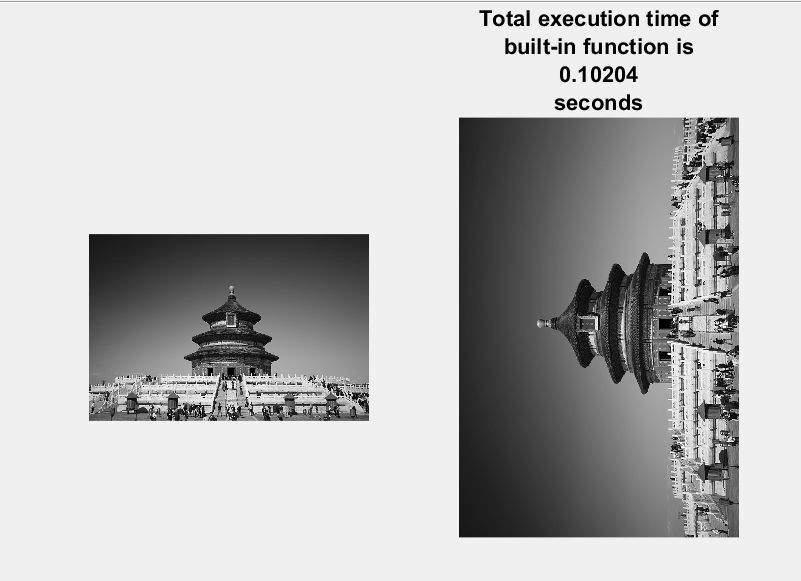
\includegraphics[width=\linewidth]{built-in-trans.png}
			\caption{Built-in rotation and execution time.}
		\end{subfigure}
	\end{figure}
	\newpage
	\begin{figure}[hbt!]
		\centering
		\begin{subfigure}[c]{0.92\linewidth}
		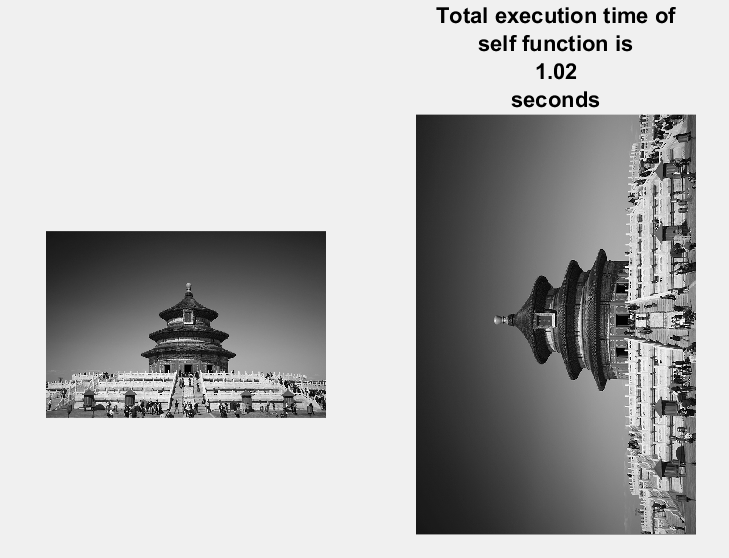
\includegraphics[width=\linewidth]{selfRot.png}
		\caption{Self-coded rotation and execution time.}
		\end{subfigure}
	\end{figure}

	\section{Histogram Equalization}
	\subsection{Code For Equalization}
	\lstinputlisting[breaklines]{histogram.m}
	\subsection{Outcome Set \RNum{2}}
	\begin{figure}[hbt!]
		\centering
			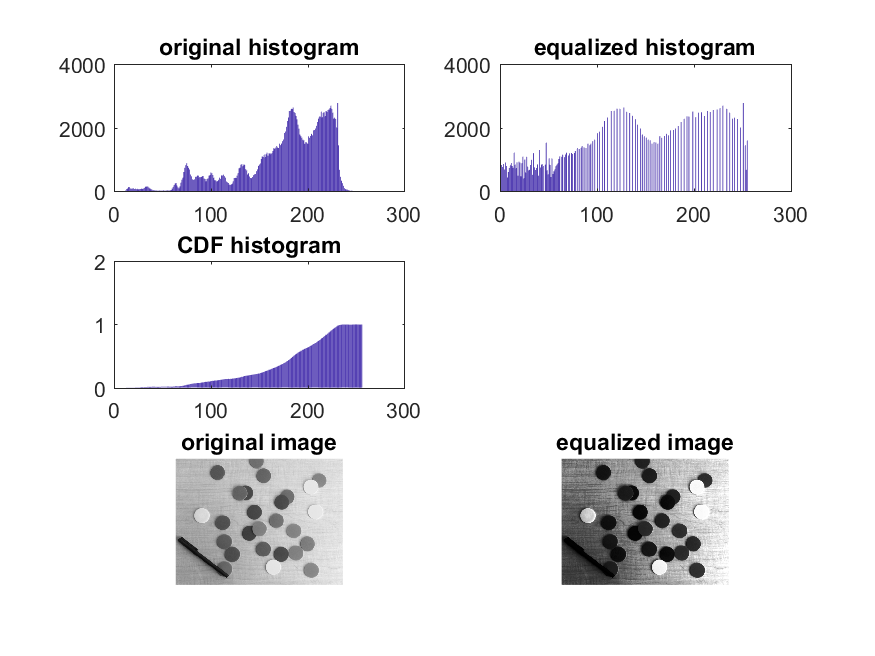
\includegraphics[width=\linewidth]{eq.png}
			\caption{Outcome of Histogram Equalization.}
	\end{figure}
	\section{Discussion}
	\subsection{Why black dots after rotation?}
	When we do a forward rotation transformation, there are many pixel not being mapped,which leads to those point unassigned with the intensity values remain 0.
	\subsection{Why the equalization not quite even?}
	This is because discretization. For the continuous transformation $ s=T(r)$ , the outcome is uniform. While for the digital image, we round the value so that there are many specific intensity value was lost.
	\subsection{Why different execution speed?}	
	From the outcome, we can see that the built-in rotation only need tenth total time of the self-coded rotation. I did not dig into the primitive implementation of built-in function such as maketform and imwarp. Definitely, it is because we implement the rotation by brute-force attack without any optimization. 

\end{document}